% !TeX root = main.tex

\section{Bayes Theorem}

This is the most important theorem for pattern recognition. It is the foundation for PR!! You will need an understanding of probabilities to understand this section.
Bayes theorem connects what we want to know with what we can measure. \autocite{duda2001}

\noindent
\textbf{exam notes:} Very important to understand and be able to reproduce for any PR exam. You should be comfortable with the terminology, the language of Pattern Recognition and applying Bayes decision rules. 
\begin{itemize}
		\item {\em \textbf{Supervised learning:}}

		      $m$ training samples, each consisting of a feature vector and its \textbf{true} class label (ground truth)
		      \begin{displaymath}
			      S = \{(\vect x_i, y_i)\}_{i=1}^m
		      \end{displaymath}
              where $\vect x_i \in \mathcal{X}$ denotes the feature vector and $y_i\in\mathcal{Y}$ denotes the \textbf{true} class label of sample $i$.
	      If nothing special is mentioned, ${\mathcal{X}}\subseteq \mathbb{R}^d$.

		\item {\em \textbf{Unsupervised learning:}}

		      $m$ training samples just include features; no class assignments and even the number of classes is (not always) known
		      \begin{displaymath}
			      S = \{ \vect x_1, \vect x_2, \vect x_3, \dots, \vect x_m \}
		      \end{displaymath}
	\end{itemize}
	
	\subsection{Notation}
	\begin{itemize}
		\item[ $\vect x \in \mathbb{R}^d:$] $d$-dimensional (observed) feature vector.
		\item[$y\in\mathcal{Y}:$] \textbf{true} class label (ground truth), e.g.\ $\mathcal{Y}=\{1,\dots,K\}$ (for binary classification often $\{0,1\}$ or $\{-1,+1\}$; stated explicitly).
		\item[$\hat y:$] \textbf{predicted} class label (output of a classifier).
		\item[$\hat y^*:$] \textbf{optimal} (Bayes) prediction.
		\item[$p(y):$] prior probability of class $y$.
		\item[$p(\vect x):$] evidence (marginal density of the features).
		\item[$p(\vect x , y):$] \textbf{joint distribution} of $(\vect x,y)$.
		\item[$p(\vect x \mid y):$] class-conditional density.
		\item[$p(y\mid \vect x):$] posterior probability.
	\end{itemize}

\noindent\textbf{Probabilities vs. densities (convention):} we use the same symbol $p(\cdot)$ for pmfs and pdfs; e.g.\ $p(y)$ is shorthand for $P(Y=y)$. A prediction is correct on sample $\vect x_i$ if $\hat y = y_i$.

\begin{figure}[H]\centering
\begin{tikzpicture}[
  box/.style={draw,rounded corners,minimum width=3.2cm,minimum height=1.1cm,align=center,font=\small},
  op/.style={circle,draw,fill=gray!15,inner sep=1pt,font=\small},
  ar/.style={-{Latex[length=2mm]},thick}]
\node[box,fill=cA!10]  (prior) {Prior $p(y)$\\[-1pt]\scriptsize ``how common is an apple?''};
\node[box,fill=cA!10,right=1.2cm of prior] (lik) {Class-conditional $p(\vect x\mid y)$\\[-1pt]\scriptsize ``how yellow are apples?''};
\node[op] (mul) at ($(prior.south)!0.5!(lik.south)+(0,-1)$) {$\times$};
\node[box,fill=gray!10,below=0.8cm of mul] (joint) {Joint $p(\vect x,y)$\\[-1pt]\scriptsize ``yellow \emph{and} apple''};
\node[op,below left=0.9cm and 1.2cm of joint] (sum) {$\sum_{y}$};
\node[box,fill=green!10,below=0.7cm of sum] (evid) {Evidence $p(\vect x)$\\[-1pt]\scriptsize ``how often is anything yellow?''};
\node[op,below right=0.9cm and 1.2cm of joint] (div) {$\div$};
\node[box,fill=cB!15,below=0.7cm of div] (post) {Posterior $p(y\mid\vect x)$\\[-1pt]\scriptsize ``apple, given it is yellow?''};
\draw[ar] (prior.south) |- (mul);
\draw[ar] (lik.south) |- (mul);
\draw[ar] (mul) -- (joint);
\draw[ar] (joint.south) -| (sum);
\draw[ar] (sum) -- node[left,font=\scriptsize]{marginalize} (evid);
\draw[ar] (joint.south) -| (div);
\draw[ar] (evid.east) -- ++(0.5,0) |- (div.west);
\draw[ar] (div) -- (post);
\end{tikzpicture}
\caption{How the probability terms of Sec.~2.1 are connected via Bayes rule.}
\end{figure}
\subsection{Bayes rule:}

	\begin{eqnarray*}
		\underbrace{p(\vect x , y)}_{\text{joint}}
		&=&   \underbrace{p(y)}_{\text{prior}} \cdot \underbrace{p(\vect x \mid y)}_{\text{class-conditional pdf}} \\
		&=& \underbrace{ p(\vect x)}_{\text{evidence}} \cdot \underbrace{ p(y\mid \vect x)}_{\text{posterior}}
	\end{eqnarray*}
	Now we get the posterior as follows:

	\begin{eqnarray*}
		p(y\mid \vect x)
		&=& \frac{p(y) \cdot p(\vect x \mid y)}{p(\vect x)} \\ 
		&=& \frac{p(y) \cdot p(\vect x \mid y)}{\sum\limits_{y'}p(\vect x , y')} \\ 
		&=& \frac{p(y) \cdot p(\vect x \mid y)}{\sum\limits_{y'}p(y') \cdot p(\vect x \mid y')}\\
	\end{eqnarray*}
	\subsubsection{Note:}
	\begin{displaymath}
		p(\vect x) = \sum\limits_{y}p(y) \cdot p(\vect x \mid y)
	\end{displaymath}
	is a \textbf{marginal} of $p(\vect x , y)$.
	\begin{itemize}
		\item We get $p(\vect{x})$ by marginalizing $p(\vect{x}, y)$ over $y$.
		\item Accordingly we get $p(y)$ by marginalizing $p(\vect{x}, y)$ over $\vect{x}$, i.\,e.
		      \begin{eqnarray*}
			      p(y)&=& \int p(\vect{x}, y) \, \mathsf{d}\vect{x}
		      \end{eqnarray*}
	\end{itemize}
	Now let us summarize the Bayesian decision rule: The optimal prediction $\hat y^*$ is the class with the highest posterior,
	\begin{eqnarray*}
		\hat y^* &=&   \argmax\limits_{y} p(y \mid \vect x) \\
		&=& \argmax_y \frac{p(y) \cdot p(\vect x \mid y)}{p(\vect x)} \\
		&=& \argmax_y p(y) \cdot p(\vect x \mid y) \\
		&=& \argmax_y\{\log p(y)\ + \log p(\vect x \mid y)\} 
	\end{eqnarray*}
	\textbf{Notes:} 
	\begin{itemize}
    \item Understand why the denominator was dropped in the above derivation. 
		\item The key aspect in designing a classifier is to find a good model for the posterior $p(y\mid\vect x)$.
		\item Feature vectors $\vect x$ usually have fixed dimension $d$ in simple classification schemes,
		\item but ${\mathcal{X}}$ is not necessarily a subset of $\mathbb{R}^d$: features of varying dimension, sequences and sets of features.
	\end{itemize}

    \begin{figure}[H]\centering
\begin{tikzpicture}[scale=0.9,transform shape]
\begin{groupplot}[group style={group size=1 by 2,vertical sep=2.0cm},
  width=9.5cm,height=4.0cm,domain=-1:8,samples=120,xmin=-1,xmax=8,
  axis lines=left,xlabel={feature $x$},every axis plot/.append style={very thick},
  legend style={draw=none,font=\scriptsize,fill=none},legend pos=north east]
\nextgroupplot[ylabel={$p(y)\,p(x\mid y)$},ymin=0,ymax=0.27,
  title={\small (a) prior $\times$ class-conditional (unnormalized)}]
 \addplot[cA] {0.6*exp(-(x-2)^2/2)/sqrt(2*pi)}; \addlegendentry{$y=0$, $p(y)=0.6$}
 \addplot[cB] {0.4*exp(-(x-5)^2/2)/sqrt(2*pi)}; \addlegendentry{$y=1$, $p(y)=0.4$}
 \draw[dashed,gray] (axis cs:3.635,0)--(axis cs:3.635,0.27);
\nextgroupplot[ylabel={$p(y\mid x)$},ymin=0,ymax=1.08,
  title={\small (b) posterior = (a) divided by evidence $p(x)$}]
 \addplot[cA] {1/(1+ (0.4*exp(-(x-5)^2/2))/(0.6*exp(-(x-2)^2/2)))}; \addlegendentry{$p(y{=}0\mid x)$}
 \addplot[cB] {1/(1+ (0.6*exp(-(x-2)^2/2))/(0.4*exp(-(x-5)^2/2)))}; \addlegendentry{$p(y{=}1\mid x)$}
 \draw[dashed,gray] (axis cs:-1,0.5)--(axis cs:8,0.5);
 \draw[dashed,gray] (axis cs:3.635,0)--(axis cs:3.635,1.08) node[pos=0.12,right,font=\scriptsize,black]{decision boundary};
\end{groupplot}
\end{tikzpicture}
\caption{Bayes rule. The posteriors always sum to one; the class with the larger $p(y)\,p(x\mid y)$ wins.}
\end{figure}

\begin{figure}[H]\centering
\begin{tikzpicture}
\begin{axis}[ybar stacked,bar width=1.1cm,width=9cm,height=6cm,ymin=0,ymax=0.45,
  xmin=0.4,xmax=3.6,xtick={1,2,3},xticklabels={green,yellow,red},
  xlabel={feature $x$ (colour)},ylabel={probability},axis lines=left,
  legend style={draw=none,font=\small,at={(1.02,0.5)},anchor=west},
  after end axis/.code={% segment labels drawn on top of the bars
   \node[font=\scriptsize,white] at (axis cs:1,0.075) {0.15};
   \node[font=\scriptsize,white] at (axis cs:2,0.075) {0.15};
   \node[font=\scriptsize,white] at (axis cs:3,0.15)  {0.30};
   \node[font=\scriptsize,white] at (axis cs:1,0.25) {0.20};
   \node[font=\scriptsize,white] at (axis cs:2,0.24) {0.18};}]
 \addplot[fill=cA,draw=none] coordinates {(1,0.15) (2,0.15) (3,0.30)};
 \addlegendentry{$p(x,\,y{=}\text{apple})$}
 \addplot[fill=cB,draw=none] coordinates {(1,0.20) (2,0.18) (3,0.02)};
 \addlegendentry{$p(x,\,y{=}\text{pear})$}
 \node[above=2pt,font=\small] at (axis cs:1,0.35) {$p(x)=0.35$};
 \node[above=2pt,font=\small] at (axis cs:2,0.33) {$0.33$};
 \node[above=2pt,font=\small] at (axis cs:3,0.32) {$0.32$};
\end{axis}
\end{tikzpicture}
\caption{Marginalization: the total bar height is $p(x)=\sum_y p(x,y)$. Summing one colour across all bars gives $p(y)$ (apple $0.6$, pear $0.4$). The posterior is a bar's segment over its total, e.g.\ $p(\text{apple}\mid\text{yellow})=0.15/0.33$.}
\end{figure}

	\subsection{Types of models}
	There are two main types of classifiers or models. 
	\begin{itemize}
		\item \textbf{Generative modeling:}  modeling and estimation of $p(y)$ and $p(\vect x | y)$. 
		Where the model tries to estimate the actual sample and hence needs knowledge of the feature space and also how to generate new samples in that feature space.
		\item \textbf{Discriminative modeling:} straight modeling and estimation of $p(y|\vect x)$. Where the model only needs to understand the difference between the two feature spaces, and does not need to know how to generate new samples. It can only discriminate between classes, cannot generate new information. 
	\end{itemize}

\noindent 
\textbf{Notes:} In this chapter, we discuss Bayesian classifiers which are generative models. The explanation of the discriminative models are given to contrast the definition only. 

\begin{figure}[H]\centering
\begin{tikzpicture}[scale=0.85,transform shape]
\def\pts{
 \foreach \x/\y in {1.0/1.2,1.5/2.0,0.6/1.8,1.9/1.4,1.2/0.7,2.2/2.3,0.8/2.6,1.7/0.9}
   {\fill[cA] (\x,\y) circle (2pt);}
 \foreach \x/\y in {3.2/2.9,3.8/3.5,3.0/3.8,4.2/2.8,3.6/2.4,4.4/3.9,2.7/3.1,3.9/4.3}
   {\fill[cB] (\x,\y) rectangle ++(4pt,4pt);}}
\begin{scope}
 \draw[-{Latex}] (0,0)--(5,0) node[below left,font=\scriptsize]{$x_1$};
 \draw[-{Latex}] (0,0)--(0,5) node[below left,font=\scriptsize]{$x_2$};
 \foreach \s in {0.5,0.9,1.3}{
  \draw[cA,rotate around={35:(1.4,1.7)}] (1.4,1.7) ellipse ({\s*1.0} and {\s*0.7});
  \draw[cB,rotate around={35:(3.6,3.4)}] (3.6,3.4) ellipse ({\s*1.0} and {\s*0.7});}
 \pts
 \node[font=\small\bfseries] at (2.5,5.6) {Generative};
 \node[font=\small,align=center] at (2.5,-0.9) {model $p(y)$ and $p(\vect x\mid y)$\\ \scriptsize ``what does each class look like?''};
\end{scope}
\begin{scope}[xshift=6.5cm]
 \fill[cA!8] (0,0)--(0,4.6)--(4.6,0)--cycle;
 \fill[cB!10] (0,4.6)--(5,4.6)--(5,0)--(4.6,0)--cycle;
 \draw[-{Latex}] (0,0)--(5,0) node[below left,font=\scriptsize]{$x_1$};
 \draw[-{Latex}] (0,0)--(0,5) node[below left,font=\scriptsize]{$x_2$};
 \draw[very thick] (0.2,4.4)--(4.4,0.2) node[pos=0.1,above right,font=\scriptsize]{$p(y\mid\vect x)=0.5$};
 \pts
 \node[font=\small\bfseries] at (2.5,5.6) {Discriminative};
 \node[font=\small,align=center] at (2.5,-0.9) {model $p(y\mid\vect x)$ directly\\ \scriptsize ``where is the border?''};
\end{scope}
\end{tikzpicture}
\caption{Same data, two strategies. Generative models describe each class (and can sample new data); discriminative models only learn the boundary.}
\end{figure}

\subsection{Optimality of the Bayesian Classifier}

A loss function quantifies the cost associated with making a decision, particularly when the decision is incorrect. Different types of classification errors may have different consequences, and the loss function allows us to express these consequences numerically. For a given decision rule, we can compute the expected loss over many samples. The best classifier is then the one that minimizes this expected loss. When all classification errors are assigned the same cost, minimizing the expected loss reduces to minimizing the classification error rate.

\begin{figure}[H]\centering
\begin{tikzpicture}
\begin{axis}[width=11cm,height=5.5cm,domain=-1:8,samples=150,xmin=-1,xmax=8,ymin=0,ymax=0.28,
  axis lines=left,xlabel={feature $x$},ylabel={$p(y)\,p(x\mid y)$},
  legend style={draw=none,font=\scriptsize,fill=none},legend pos=north east]
 \addplot[cA,very thick,name path=A] {0.6*exp(-(x-2)^2/2)/sqrt(2*pi)}; \addlegendentry{$y=0$}
 \addplot[cB,very thick,name path=B] {0.4*exp(-(x-5)^2/2)/sqrt(2*pi)}; \addlegendentry{$y=1$}
 \path[name path=ax] (axis cs:-1,0)--(axis cs:8,0);
 \addplot[cB!40] fill between[of=B and ax,soft clip={domain=-1:3.635}];
 \addplot[cA!40] fill between[of=A and ax,soft clip={domain=3.635:8}];
 \draw[thick,dashed] (axis cs:3.635,0)--(axis cs:3.635,0.27) node[above,font=\scriptsize]{$x^*$};
 \node[font=\scriptsize,cA] at (axis cs:1,0.25) {decide $\hat y^*=0$};
 \node[font=\scriptsize,cB] at (axis cs:6.3,0.19) {decide $\hat y^*=1$};
 \node[font=\scriptsize,align=center] (e) at (axis cs:5.6,0.11) {shaded = error\\(0,1)-loss $=1$};
 \draw[-{Latex},thin] (e.south west)--(axis cs:4.0,0.02);
 \draw[-{Latex},thin] (e.west)--(axis cs:3.3,0.025);
\end{axis}
\end{tikzpicture}
\caption{The Bayes classifier $\hat y^*=\arg\max_y p(y\mid\vect x)$ places the boundary where the curves cross. $x^*$ is the crossing point, i.\,e.\ the decision boundary. Moving it in either direction only adds shaded area, so no other rule has a lower expected (0,1)-loss.}
\end{figure}
	
$l(y',y)$ is the \textbf{loss} of assigning true class $y$ to class $y'$. The $(0,1)$-loss function is defined by
		\begin{eqnarray*}
			l(y',y) &= &\left\{ \begin{array}{ll}
				0 & \text{if } y'=y \\
				1 & \text{otherwise}
			\end{array} \right.
		\end{eqnarray*}

\noindent
The \textbf{best (optimal) decision rule} minimizes the expected loss
\begin{eqnarray*}
	\mathsf{AL}(\vect x , y') &=& \sum\limits_{y} l(y',y)\,p(y\mid\vect x),
\end{eqnarray*}
where the true class is unknown, so we average over its posterior.

Using the $(0,1)$-loss, the optimal prediction is
	\begin{eqnarray*}
		\hat y^* &=& \argmin\limits_{y'} \mathsf{AL}(\vect x, y')\\
		        &=& \argmin\limits_{y'} \left(1-p(y'\mid\vect x)\right)\\ 
		        &=& \argmax\limits_{y'} p(y'\mid\vect x).\\
	\end{eqnarray*}
	
	\subsection{Conclusion}

	\begin{itemize}
		\item The optimal classifier w.\,r.\,t.\ the (0,1)-loss function applies the Bayesian decision rule.
		\item This classifier is called \textbf{Bayesian classifier}. The Bayesian classifier is an ideal classifier that is mostly impossible to achieve in reality.  
	\end{itemize}
	

    \noindent
    \vorsicht The $(0,1)$-loss function is {\bf NOT} convex. Hence optimizing this loss function in practical scenario is very difficult 

\begin{figure}[H]\centering
\begin{tikzpicture}[scale=0.85,transform shape]
\begin{axis}[name=l,width=0.46\linewidth,height=0.34\linewidth,xmin=-3,xmax=3,ymin=0,ymax=3.2,axis lines=left,
  xlabel={margin $y\,F(\vect x)$},ylabel={loss},title={\small (a) (0,1)-loss vs.\ convex surrogate},
  legend style={draw=none,font=\scriptsize,fill=none},legend pos=north east]
 \addplot[black,very thick,const plot] coordinates {(-3,1) (0,1) (0,0) (3,0)}; \addlegendentry{(0,1)-loss}
 \addplot[cB,very thick,domain=-3:3,samples=80] {ln(1+exp(-x))/ln(2)}; \addlegendentry{logistic}
 \node[font=\scriptsize,align=center] at (axis cs:-1.4,0.45) {flat: zero gradient};
\end{axis}
\begin{axis}[at={(l.east)},anchor=west,xshift=0.04\linewidth,width=0.50\linewidth,height=0.38\linewidth,view={-35}{40},
  domain=-3:3,y domain=-3:3,samples=35,colormap/viridis,
  xlabel={$\theta_1$},ylabel={$\theta_2$},zlabel={loss},ticks=none,
  title={\small (b) non-convex landscape}]
 \addplot3[surf,shader=interp,opacity=0.9]
   {0.15*(x^2+y^2) - 1.3*exp(-((x-1.3)^2+(y-1.2)^2)) - 0.8*exp(-((x+1.4)^2+(y+0.9)^2)/0.8) - 0.6*exp(-((x+1)^2+(y-1.6)^2)/0.6)};
\end{axis}
\end{tikzpicture}
\caption{(a) The (0,1)-loss is a step: non-convex with zero gradient almost everywhere, so it cannot be minimized by gradient methods. (b) A non-convex landscape has several local minima; the result depends on initialization.}
\end{figure}

	\subsection{Lessons Learned}
\begin{itemize}
		\item General structure of a classification system 
		\item Supervised and unsupervised learning  
		\item Basics on probabilities (probability, pdf, Bayes rule, etc.)  
		\item Optimality of Bayes classifier and the role of the loss function   
		\item Discriminative and generative approach to model a posteriori probability
	\end{itemize}

\clearpage

\newpage

\section{Logistic regression}

Despite its name, logistic regression is a \textbf{classification} method: it models the posterior $p(y\mid\vect x)$ directly by a logistic (sigmoid) function, and its parameters are estimated by maximizing the log-likelihood (Sec.~\ref{sec:lr_learning}). The name comes from regressing the log-odds on the features. Compare: in \emph{regression} a continuous value is predicted (e.g.\ the exact size of a flower), in \emph{classification} only the class (flower A or B).\autocite{hastie2009,bishop2006}

\subsection{Posteriors and the Logistic Function}

\begin{figure}
    \centering
    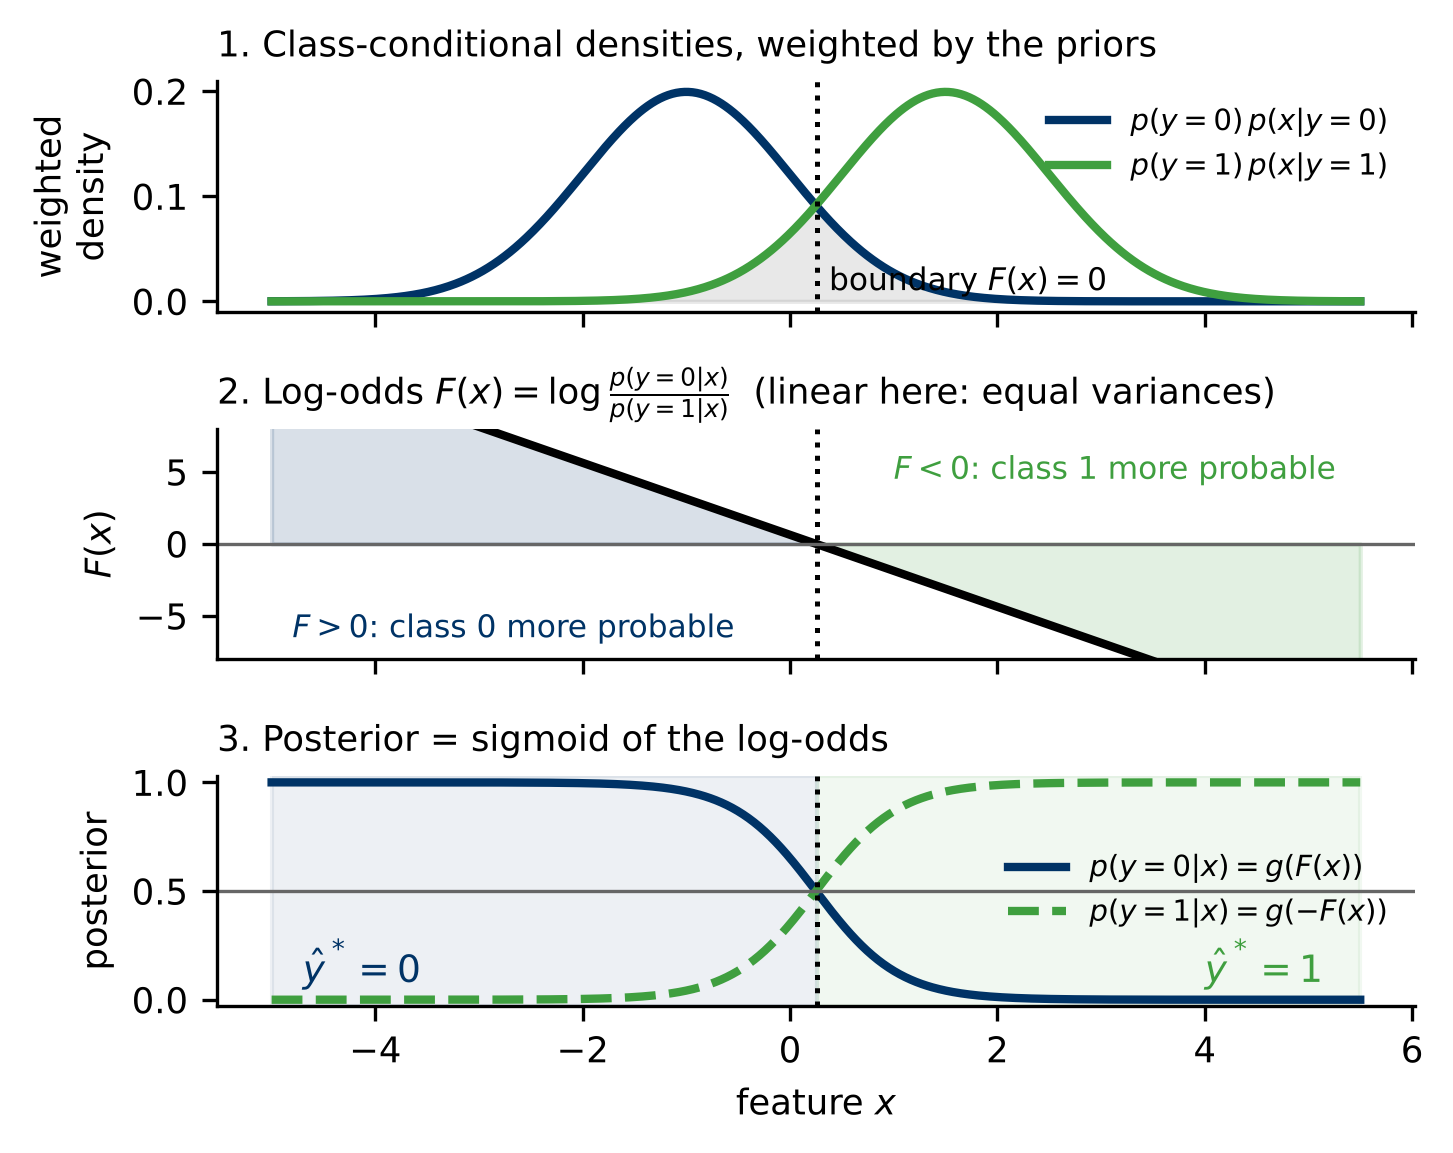
\includegraphics[width=0.75\linewidth]{ch03_densities_logodds_posterior.png}
    \caption{From class-conditional densities to the posterior for 1-D Gaussians with $\mu_0=-1$, $\mu_1=1.5$, $\sigma=1$, equal priors.}
    \label{fig:logodds_posterior}
\end{figure}

For two classes $y\in\{0, 1\}$ we get:
  
  \begin{eqnarray*}
    p(y=0\mid \vect x)
      &=&  \frac{p(y=0)\, p(\vect x \mid y=0)}{p(\vect x)} \\ 
      &=& \frac{p(y=0)\, p(\vect x \mid y=0)}{p(y=0)p(\vect x \mid y=0)+p(y=1)p(\vect x \mid y=1)} \\
      &=& \frac{1}{1+\frac{p(y=1)p(\vect x\mid y=1)}{p(y=0)p(\vect x\mid y=0)}} \\
      &\phantom{=}& \mbox{\small (\textbf{Trick:} extend with exponential and logarithm)} \\ 
      &=& \frac{1}{1+e^{\log \frac{p(y=1)p(\vect x\mid y=1)}{p(y=0)p(\vect x\mid y=0)}}} \\
      &=& \frac{1}{1+e^{-\log\frac{p(y=0)}{p(y=1)} - \log\frac{p(\vect x\mid y=0)}{p(\vect x\mid y=1)}}}\\
      &=& \frac{1}{1+e^{-\log\frac{p(y=0\mid\vect x)}{p(y=1\mid\vect x)}}}.
  \end{eqnarray*}
 We see that the posterior for class $y = 0$ can be written in terms of a \textbf{logistic function}. Define
\begin{eqnarray*}
  F(\vect x) := \log\frac{p(y=0\mid\vect x)}{p(y=1\mid\vect x)}
\end{eqnarray*}
(i.e.\ $F$ is the log-odds of class $0$ vs.\ class $1$). Then
 \begin{eqnarray*}
    p(y=0\mid \vect x) &=& \frac{1}{1+e^{-F(\vect{x})}}.
  \end{eqnarray*}
  And thus the posterior for the other class $y = 1$:
  \begin{eqnarray*}
    p(y=1\mid \vect x) &=& 1- p(y=0\mid \vect x) \\
                   &=& \frac{e^{-F(\vect x)}}{1+e^{-F(\vect{x})}} \\
                   &=&  \frac{1}{1+e^{F(\vect{x})}}.
  \end{eqnarray*}
The {\em logistic function} (also called {\em sigmoid function}) is defined by
    \begin{eqnarray*}
      g(z) &=& \frac{1}{1+e^{-z}},
    \end{eqnarray*}
    where $z\in \mathbb{R}$ (a scalar, not a feature vector).
    
The reason we have transformed into this kind of logistic or sigmoid function, is because it fulfills this nice derivative property which will help us in the following chapters. The derivative is given by:
  \begin{eqnarray*}
    g'(z) &=& \left( \frac{1}{1+e^{-z}} \right)' = \left( (1+e^{-z})^{-1}\right)'=  \frac{1}{(1+e^{-z})^2}\cdot e^{-z} \\ 
          &=& \frac{1}{(1+e^{-z})} \cdot \frac{e^{-z}}{(1+e^{-z})} \\
          &=& \frac{1}{(1+e^{-z})} \cdot \frac{1}{(1+e^{z})} \\
          &=& g(z)g(-z) \\
          &=& g(z)(1-g(z)) \quad.
  \end{eqnarray*}

  \begin{figure}
      \centering
      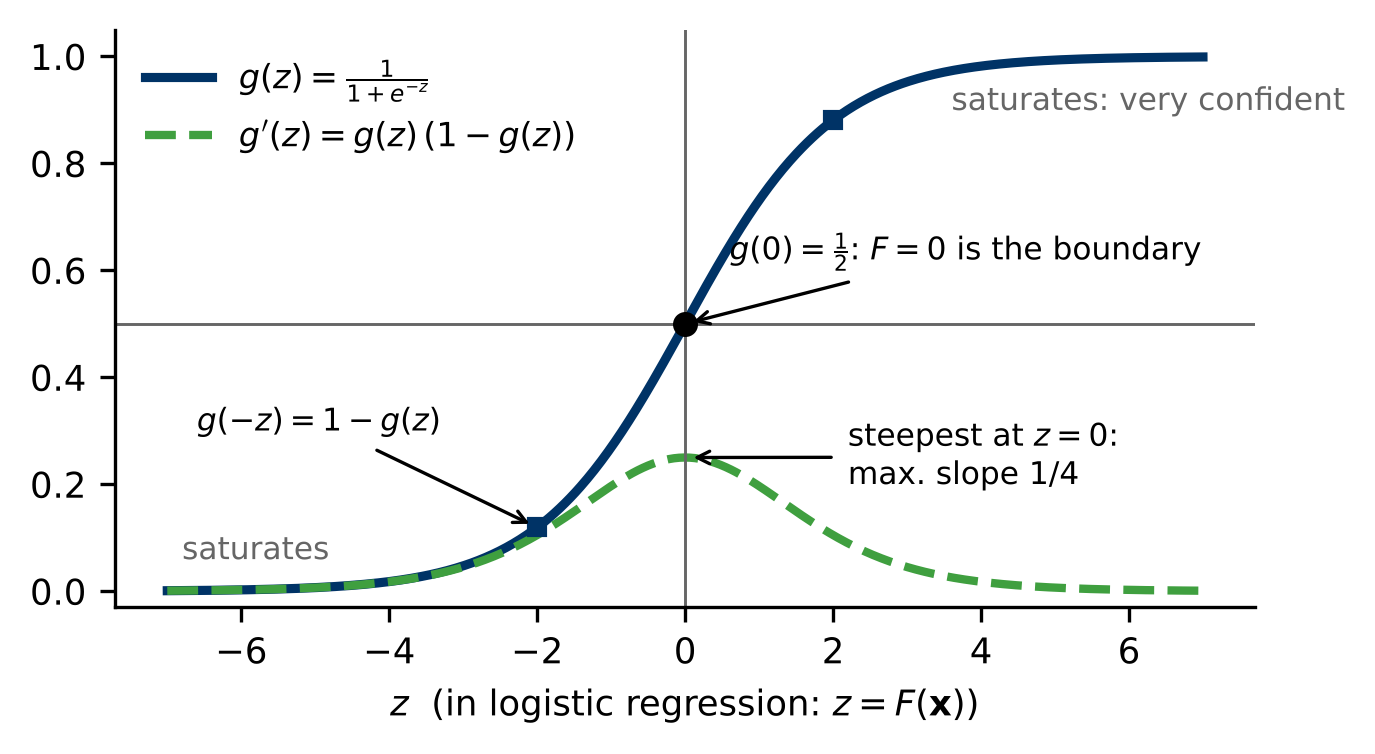
\includegraphics[width=0.75\linewidth]{ch03_sigmoid_properties.png}
      \caption{Logistic (sigmoid) function $g(z)=\frac{1}{1+e^{-z}}$ and its derivative $g'(z)=g(z)(1-g(z))$.}
      \label{fig:sigmoid_properties}
  \end{figure}
  \subsection{Decision Boundary}
    The \textbf{decision boundary} in feature space separates the regions where the classifier decides for class $0$ and class $1$. On the boundary, the posterior probabilities are equal; for the two-class case this means $p(y=0\mid\vect x)=p(y=1\mid\vect x)=0.5$.
  Points $\vect x$ on the decision boundary satisfy:
 
  \begin{eqnarray*}
    {p(y=0|\vect{x})}&=& {p(y=1|\vect x)}
  \end{eqnarray*}
  and thus
  \begin{eqnarray*}
    \log \frac{p(y=0|\vect{x})}{p(y=1|\vect x)} &=& \log 1 = 0 \quad.
  \end{eqnarray*}
  The lemma below makes the decision-boundary condition explicit.
  \begin{lemma}
    The decision boundary is given by $F(\vect x)=0$.
  \end{lemma}
  \textbf{Proof:} By definition, $F(\vect x)=\log\frac{p(y=0\mid\vect x)}{p(y=1\mid\vect x)}$. Hence
  \begin{eqnarray*}
    F(\vect x)=0
    &\Leftrightarrow& \log\frac{p(y=0\mid\vect x)}{p(y=1\mid\vect x)}=0 \\
    &\Leftrightarrow& \frac{p(y=0\mid\vect x)}{p(y=1\mid\vect x)}=1 \\
    &\Leftrightarrow& p(y=0\mid\vect x)=p(y=1\mid\vect x).
  \end{eqnarray*}

  Since $p(y=0\mid\vect x)+p(y=1\mid\vect x)=1$, we get $p(y=0\mid\vect x)=p(y=1\mid\vect x)=\tfrac{1}{2}$ if and only if $F(\vect x)=0$.


  \subsection{Decision Rule}
  The classifier predicts class $0$ if the posterior of class $0$ is larger than $\tfrac{1}{2}$, i.\,e. if $F(\vect x)>0$:
  \begin{eqnarray*}
    \hat y^* &=& \left\{\begin{array}{ll}
      0 & \text{if } F(\vect x) > 0 \\
      1 & \text{if } F(\vect x) < 0
    \end{array}\right.
  \end{eqnarray*}
  The boundary is given by $F(\vect x)=0$. Note that $\hat y^*$ is the predicted class; the true class $y$ (or labels $y_i$ in the training set) can differ.

\begin{figure}
    \centering
    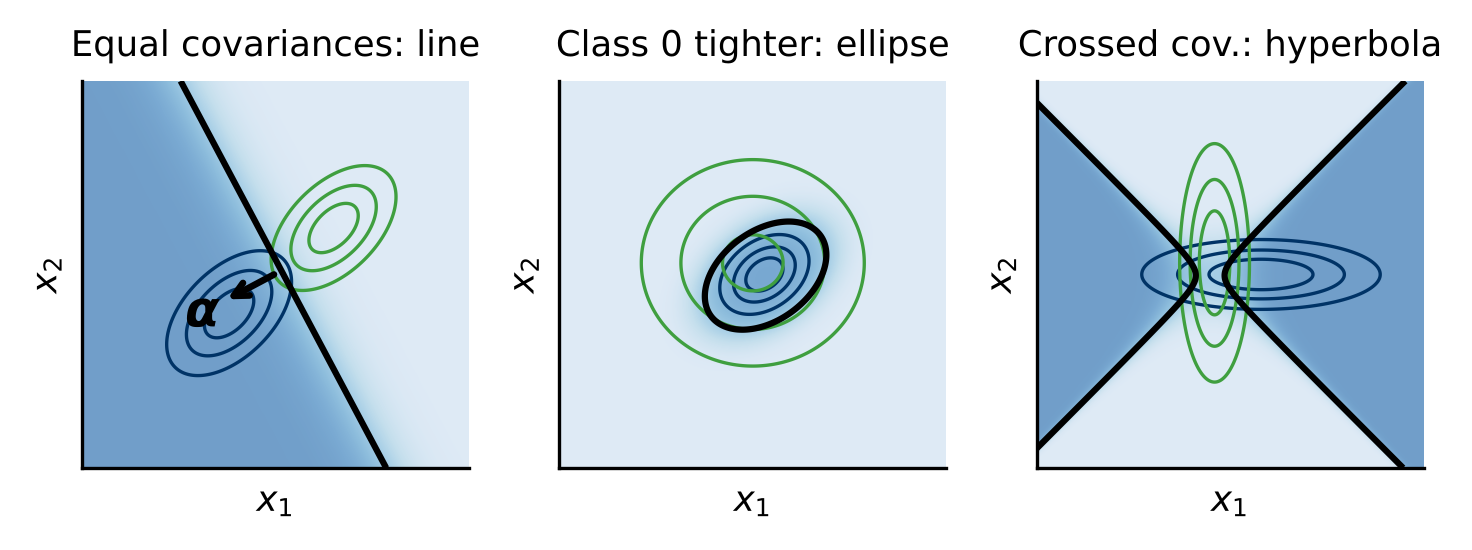
\includegraphics[width=0.8\linewidth]{ch03_2d_boundaries.png}
    \caption{Decision boundaries $F(\vect x)=0$ for two 2-D Gaussian classes: equal covariances give a line; unequal covariances give conic sections.}
    \label{fig:boundaries}
\end{figure}
 \subsubsection{Example}
    \textbf{Note:} Important to understand this example and derivation. Forms the foundation of future chapters. Let us assume both classes have normally distributed $d$-dimensional feature vectors:
    \begin{eqnarray*}
      p(\vect x \mid y) &=& \mathcal N(\vect x;\vect\mu_y,\mat\Sigma_y)
      = \frac{1}{\sqrt{\det(2\pi \mat\Sigma_y)}}
        e^{-\frac{1}{2} (\vect{x} - \vect{\mu}_y)^T \mat\Sigma_y^{-1} (\vect{x} - \vect{\mu}_y)}
    \end{eqnarray*}
    where $\mat\Sigma_y$ is the covariance matrix and $\vect\mu_y$ the mean of class $y$. This convention is followed throughout the document. 
 
    Then we can write the posterior of $y=0$ in terms of a logistic function:
 
    \begin{eqnarray*}
      p(y=0|\vect x) &=& \frac{1}{1+e^{-F(\vect x)}} = \frac{1}{1+e^{ - \left( \vect x^T \mat A \vect x + \vect \alpha^T\vect x + \alpha_0 \right) } } \\ \\
      F(\vect x) &=& \log \frac{p(y=0|\vect x)}{p(y=1|\vect x)} = \log \frac{p(y=0)p(\vect x | y=0) }{p(y=1)p(\vect x|y =1)}\\
      F(\vect x) &=&
        \log\frac{p(y=0)}{p(y=1)} +
        \log
        \frac{
          \frac{1}{ \sqrt{ \det{( 2 \pi \mat{\Sigma}_0)}} }
          e^{ -\frac{1}{2} (\vect{x} - \vect{\mu}_0)^T \mat{\Sigma}_0^{-1} (\vect{x} - \vect{\mu}_0) }         
        }{
          \frac{1}{ \sqrt{ \det{(2 \pi \mat{\Sigma}_1)}} }
          e^{ -\frac{1}{2} (\vect{x} - \vect{\mu}_1)^T \mat{\Sigma}_1^{-1} (\vect{x} - \vect{\mu}_1)}
        }
    \end{eqnarray*}
  This function has the constant component (it becomes part of $\alpha_0$ below):
% 
    \begin{eqnarray*}
      \log \frac{p(y=0)}{p(y=1)}+\frac{1}{2}
            \log \frac{ { \det{(2\pi\mat{\Sigma}_1)}}}
                      { { \det{(2\pi\mat{\Sigma}_0)}}}
    \end{eqnarray*}
     We observe:
    \begin{itemize}
      \small
      \item Priors imply a constant offset of the decision boundary. 
      \item If priors and covariance matrices of both classes are identical, this offset is $0$.
    \end{itemize}

   \begin{figure}
       \centering
       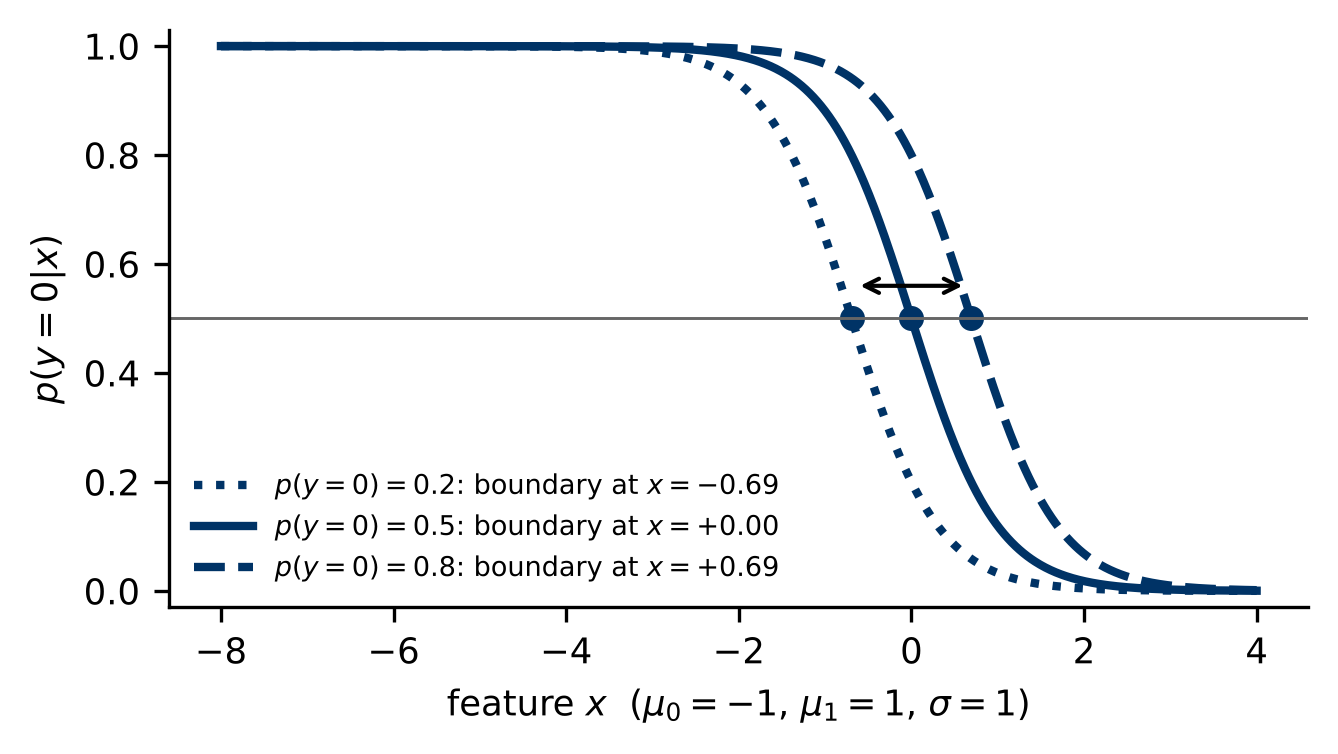
\includegraphics[width=0.75\linewidth]{ch03_prior_shift.png}
       \caption{Effect of the prior on the decision boundary for 1-D Gaussians with $\mu_0=-1$, $\mu_1=1$, $\sigma=1$. Changing $p(y=0)$ shifts the posterior and moves the decision boundary.}
       \label{fig:prior_shift}
   \end{figure}
   Furthermore we have:
    {\small
    \begin{eqnarray*}
      \log{ 
        \frac{e^{ - \frac{1}{2} (\vect{x} - \vect{\mu}_0)^T \mat{\Sigma}_0^{-1} (\vect{x} - \vect{\mu}_0)} }
             {e^{ - \frac{1}{2} (\vect{x} - \vect{\mu}_1)^T \mat{\Sigma}_1^{-1} (\vect{x} - \vect{\mu}_1)} }
      } & = & 
      \frac{1}{2} 
      \left(
        (\vect{x} - \vect{\mu}_1)^T \mat{\Sigma}_1^{-1} (\vect{x} - \vect{\mu}_1) - (\vect{x} - \vect{\mu}_0)^T \mat{\Sigma}_0^{-1} (\vect{x} - \vect{\mu}_0)
      \right) \\
      & &  =
      \frac{1}{2} 
      \left(
        \vect{x}^T (\mat{\Sigma}_1^{-1} - \mat{\Sigma}_0^{-1}) \vect{x} 
        -2 (\vect{\mu}_1^T \mat{\Sigma}_1^{-1} - \vect{\mu}_0^T \mat{\Sigma}_0^{-1} ) \vect{x} + \right.\\
        & & \left.  
        + \vect{\mu}_1^T \mat{\Sigma}_1^{-1} \vect{\mu}_1 - \vect{\mu}_0^T \mat{\Sigma}_0^{-1} \vect{\mu}_0
      \right)
    \end{eqnarray*}
    }
     Now we have:
    \begin{eqnarray*}
      \mat{A}        &=& \frac{1}{2} (\mat{\Sigma}_1^{-1} - \mat{\Sigma}_0^{-1}) \\[.5cm]
      \vect{\alpha}^T &=& \vect{\mu}_0^T \mat{\Sigma}_0^{-1} - \vect{\mu}_1^T \mat{\Sigma}_1^{-1} \\
      \alpha_0       &=& \log \frac{p(y=0)}{p(y=1)} + \frac{1}{2}
                         \left(
                           \log
                             \frac{ \det{( 2 \pi \mat{\Sigma}_1)}}
                                  { \det{( 2 \pi \mat{\Sigma}_0)}} + 
                             \vect{\mu}_1^T \mat{\Sigma}_1^{-1} \vect{\mu}_1 -
                             \vect{\mu}_0^T \mat{\Sigma}_0^{-1} \vect{\mu}_0
                         \right)
    \end{eqnarray*}
    \subsubsection{Properties}
    Quadratic polynomials in the 2 variables $x_1$ and $x_2$\\
    This means if the two variables have a quadratic polynomial relationship with each other. This section is important to understand. 
    
   \begin{eqnarray*}
    F(\vect{x}) 
      &=& \vect x^T \mat A \vect x + \vect \alpha^T\vect x + \alpha_0 \\
      &=& a_{11}x_1^2 + (a_{12}+a_{21})x_1x_2 + a_{22}x_2^2 + \alpha_1 x_1 + \alpha_2 x_2 + \alpha_0 \stackrel{!}{=} 0
  \end{eqnarray*}\\
  \textbf{Posterior probability: } 
  The posterior probability impacts the decision boundary. Below is some of the impacts explained. \\
  
  \subsubsection{Distributions with Equal Dispersion}
    If both classes share the same covariance, i.\,e.\ $\mat\Sigma= \mat\Sigma_0=\mat\Sigma_1$, then the argument $F(\vect x)$ of the sigmoid function is \textbf{affine} in $\vect{x}$.
    \begin{eqnarray*}
      \mat{A}        &=& \mat{0} \\
      \vect{\alpha}^T &=& (\vect{\mu}_0 - \vect{\mu}_1)^T \mat{\Sigma}^{-1} \\
      \alpha_0       &=& \log \frac{p(y=0)}{p(y=1)} +
                         \frac{1}{2}(\vect{\mu}_1 + \vect{\mu}_0)^T \mat{\Sigma}^{-1} (\vect{\mu}_1 - \vect{\mu}_0)
     \end{eqnarray*}
\textbf{Note:}
  \begin{itemize}
    \item If the class conditionals are Gaussians and share the same covariance, the argument of the exponential function is affine in $\vect x$.
    \item This result is even true for a more general family of pdfs and not limited to Gaussians.
  \end{itemize}
 \textbf{Definition}
The {\em exponential family} is a class of pdfs that can be written in the following canonical form
    \begin{eqnarray*}
      p(\vect x;\vect \eta, \phi) &=& e^{\frac{\vect\eta^T \cdot \vect  x -b(\vect \eta)}{a(\phi)}+c(\vect x,\phi)}
    \end{eqnarray*}
    where $\vect \eta\in \mathbb{R}^d$ is the \emph{natural (canonical) parameter vector}, and $\phi$ is the {\em dispersion parameter}. \\
    \textbf{Notation:} parameters are written after \texttt{;} (e.g.\ $p(\vect x;\vect\eta)$), while conditioning uses $\mid$ (e.g.\ $p(\vect x\mid y)$).
  
  \subsubsection{Exponential family of density functions}
  
  When the class-conditional densities $p(\vect x\mid y=0)$ and $p(\vect x\mid y=1)$ belong to the \emph{same} exponential family and share the same dispersion parameter $\phi$, then the log-odds (and hence the decision boundary) is linear in $\vect x$ (see Lemma~2).
  
  \begin{itemize}
      \item {Gaussian probability density function:}
      The class-conditional density for a Gaussian is:
      
     \begin{displaymath}
    \mathcal{N}(\vect{x}; \vect{\mu},\mat{\Sigma}) = \frac{1}{ \sqrt{ \det{(2 \pi \mat{\Sigma})} } }
                    e^{-\frac{1}{2} (\vect{x} - \vect{\mu})^T \mat{\Sigma}^{-1} (\vect{x} - \vect{\mu})  } 
  \end{displaymath}
  \item {Exponential density:}
   \begin{displaymath}
    p(x;\lambda) = \left\{ 
                 \begin{array}{ll}
                   \lambda e^{-\lambda x} & x \ge 0 \\
                   0                      & x < 0 \\
                 \end{array}
               \right.
  \end{displaymath}
  \item {Binomial pmf (success probability $\pi$):}
  \begin{displaymath}
    p(k;n,\pi) = \binom{n}{k} \pi^k (1-\pi)^{n-k}
  \end{displaymath}
  \item {Poisson pmf:}
  \begin{displaymath}
    p(k;\lambda) = \frac{\lambda^k}{k!} e^{-\lambda}
  \end{displaymath}
  \item {Hypergeometric pmf:}
  \begin{displaymath}
    p(k;N,M,n) = \frac{\binom{M}{k}\binom{N-M}{n-k}}{\binom{N}{n}}
  \end{displaymath}
  \end{itemize}

   \begin{lemma}
     If all class-conditional densities are members of the same exponential family of probability density functions with equal dispersion $\phi$, the decision boundary $F(\vect{x})=0$ is linear in the components of $\vect{x}$.
   \end{lemma}
   
   \subsection{Lessons Learned}

  \begin{itemize}
    \item Posteriors can be rewritten in terms of a logistic function. 
    \item Given the decision boundary $F(\vect x)=0$, we can write down the posterior $p(y|\vect x)$ right away.
    \item With class-specific Gaussian covariances, the decision boundary $F(\vect x)=0$ is quadratic in $\vect x$ (a conic section in $d=2$, and a quadric surface in higher dimensions).
    \item If the Gaussian classes share the same covariance matrix, then $F(\vect x)=0$ is linear in $\vect x$, i.e.\ a hyperplane (a straight line only for $d=2$).

\begin{figure}
    \centering
    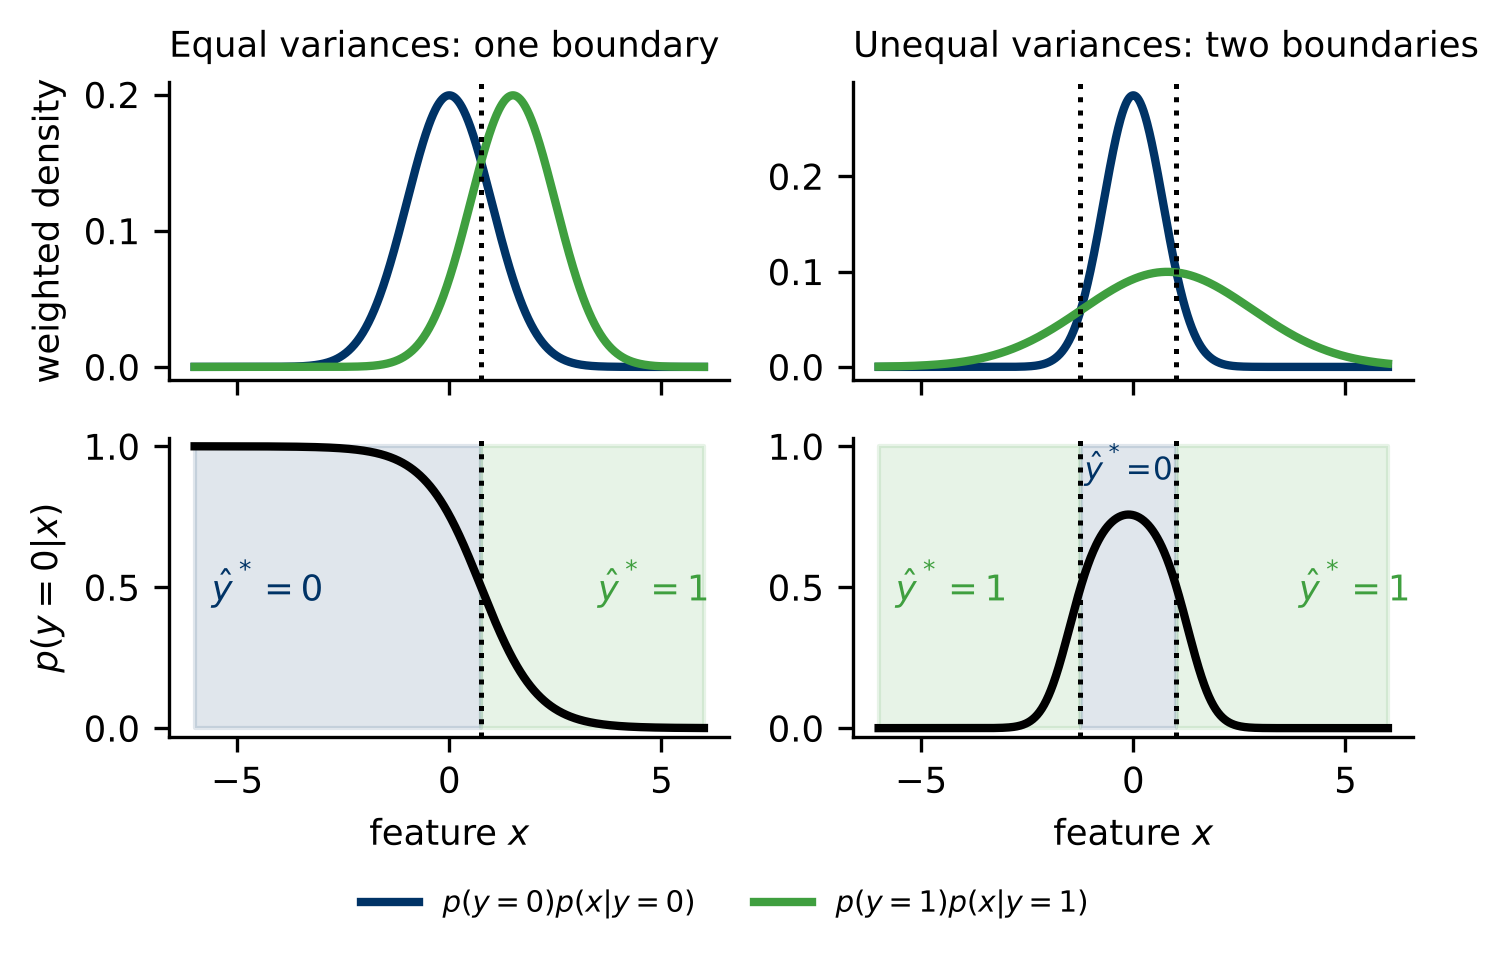
\includegraphics[width=0.75\linewidth]{ch03_equal_vs_unequal_variance.png}
    \caption{Equal vs. unequal variances in 1-D (equal priors): with equal variances $F(x)$ is linear; with unequal variances $F(x)$ is quadratic (and can yield two decision boundaries).}
    \label{fig:unequal_covariances}
\end{figure}
  \end{itemize}
  
\subsection{Parameterization}

Need understanding of linear algebra for this section. 

 \begin{itemize}
    \item Until now, $F(\vect x)$ was some arbitrary function in $\vect x$ \\[.1cm]
      \textbf{Example:} $ F(\vect x) = \vect x^T \mat A \vect x + \vect \alpha^T\vect x + \alpha_0 $ \\[.25cm]
    \item We can express a nonlinear $F(\vect x)$ as a scalar product by lifting $\vect x$ into a higher dimensional space. \\
      Given \\
     $\vect x = \left(x_1, x_2\right)^T \in \real^2,~ \mat A = \left( \begin{array}{cc} a_{11} & a_{12} \\ a_{21} & a_{22} \end{array} \right), ~ \vect \alpha = \left(\alpha_1, \alpha_2 \right)^T, ~\alpha_0 $\,, \\
      then \\
      $F(\vect x) = a_{11} x_1^2 + (a_{12} + a_{21}) x_1 x_2 + a_{22} x_2^2 + \alpha_1 x_1 + \alpha_2 x_2 + \alpha_0$\,.\\[.25cm]
    \item Rewrite $F(\vect x)=\vect a^T\vect x'$ with $\vect a,\vect x' \in \real^6$:
      \\
       $\vect a = (a_{11}, a_{12} + a_{21}, a_{22}, \alpha_1, \alpha_2, \alpha_0)^T$ \\
      $\vect x' = ( x_1^2, x_1 x_2, x_2^2, x_1, x_2, 1)^T$
  \end{itemize}

\begin{figure}[htbp]
  \centering
  \begin{tikzpicture}
  \begin{groupplot}[group style={group size=2 by 1,horizontal sep=1.2cm},
    width=5.6cm,height=4.8cm,xmin=-2.4,xmax=2.4,axis lines=middle,
    every axis plot/.append style={mark size=2.2pt},
    tick label style={font=\tiny},label style={font=\scriptsize},title style={font=\small}]
  \nextgroupplot[ymin=-0.6,ymax=0.6,ytick=\empty,xlabel={$x$},
    title={original: $x\in\mathbb{R}$}]
   \addplot[cA,only marks,mark=*] coordinates {(-0.8,0) (-0.4,0) (0,0) (0.3,0) (0.7,0)};
   \addplot[cB,only marks,mark=square*] coordinates {(-2,0) (-1.6,0) (-1.3,0) (1.3,0) (1.7,0) (2.1,0)};
   \node[font=\scriptsize,align=center] at (axis cs:0,-0.35) {no single threshold works};
   \draw[dashed,gray] (axis cs:-1,-0.25)--(axis cs:-1,0.25);
   \draw[dashed,gray] (axis cs:1,-0.25)--(axis cs:1,0.25);
  \nextgroupplot[ymin=-0.3,ymax=4.8,xlabel={$x$},ylabel={$x^2$},
    title={lifted: $\varphi(x)=(x,\,x^2)$}]
   \addplot[gray,thin,no marks,domain=-2.2:2.2,samples=60] {x^2};
   \addplot[cA,only marks,mark=*] coordinates {(-0.8,0.64) (-0.4,0.16) (0,0) (0.3,0.09) (0.7,0.49)};
   \addplot[cB,only marks,mark=square*] coordinates {(-2,4) (-1.6,2.56) (-1.3,1.69) (1.3,1.69) (1.7,2.89) (2.1,4.41)};
   \draw[very thick] (axis cs:-2.4,1)--(axis cs:2.4,1)
     node[pos=0.02,above right,font=\scriptsize,fill=white,inner sep=1pt]{$x^2=1$};
  \end{groupplot}
  \end{tikzpicture}

  \caption{Lifting in 1D: $F(x)=\alpha_0+\alpha_1x+\alpha_2x^2$ is quadratic in $x$, but linear in the lifted features $\varphi(x)=(x,\,x^2)$.}
  \label{fig:lifting_1d_quadratic_to_linear}
\end{figure}

\begin{figure}[htbp]
  \centering
  \begin{tikzpicture}
  \begin{axis}[name=flat,width=5cm,height=5cm,axis equal image,xmin=-2.1,xmax=2.1,ymin=-2.1,ymax=2.1,
    axis lines=middle,ticks=none,xlabel={$x_1$},ylabel={$x_2$},label style={font=\scriptsize},
    title={original: not linearly separable},title style={font=\small},
    every axis plot/.append style={only marks,mark size=2pt}]
   \addplot[cA,mark=*] coordinates {(0.52,-0.06) (0.47,0.31) (0.06,0.23) (-0.08,0.7) (-0.26,0.23) (-0.47,-0.09) (-0.35,-0.34) (-0.07,-0.28) (0.26,-0.67) (0.53,-0.37)};
   \addplot[cB,mark=square*] coordinates {(1.42,0.1) (1.44,0.78) (1.07,0.92) (0.39,1.54) (-0.15,1.74) (-0.81,1.57) (-1.16,1.27) (-1.62,0.72) (-1.42,-0.22) (-1.44,-0.36) (-0.89,-1.3) (-0.51,-1.43) (0,-1.55) (0.53,-1.54) (1.29,-1.2) (1.68,-0.56)};
   \draw[dashed,thick] (axis cs:0,0) circle[radius=1.1];
  \end{axis}
  \begin{axis}[at={(flat.east)},anchor=west,xshift=0.6cm,width=6.3cm,height=6cm,view={30}{20},
    xmin=-2,xmax=2,ymin=-2,ymax=2,zmin=0,zmax=3.6,ticks=none,
    xlabel={$x_1$},ylabel={$x_2$},label style={font=\scriptsize},
    title={lifted: $z=x_1^2+x_2^2$},title style={font=\small}]
   \addplot3[mesh,gray!45,domain=0:1.85,y domain=0:360,samples=10,samples y=25,z buffer=sort]
     ({x*cos(y)},{x*sin(y)},{x^2});
   \addplot3[surf,shader=flat,draw=gray!60,opacity=0.5,colormap={flat}{color=(gray!35) color=(gray!35)},domain=-2:2,y domain=-2:2,samples=2] {1.2};
   \addplot3[cA,only marks,mark=*,mark size=2pt] coordinates {(0.52,-0.06,0.27) (0.47,0.31,0.32) (0.06,0.23,0.06) (-0.08,0.7,0.5) (-0.26,0.23,0.12) (-0.47,-0.09,0.23) (-0.35,-0.34,0.24) (-0.07,-0.28,0.08) (0.26,-0.67,0.52) (0.53,-0.37,0.42)};
   \addplot3[cB,only marks,mark=square*,mark size=2pt] coordinates {(1.42,0.1,2.03) (1.44,0.78,2.68) (1.07,0.92,1.99) (0.39,1.54,2.52) (-0.15,1.74,3.05) (-0.81,1.57,3.12) (-1.16,1.27,2.96) (-1.62,0.72,3.14) (-1.42,-0.22,2.06) (-1.44,-0.36,2.2) (-0.89,-1.3,2.48) (-0.51,-1.43,2.3) (0,-1.55,2.4) (0.53,-1.54,2.65) (1.29,-1.2,3.1) (1.68,-0.56,3.14)};
  \end{axis}
  \end{tikzpicture}
  \caption{Lifting in 2D: with $\varphi(\vect x)=(x_1,\,x_2,\,x_1^2+x_2^2)$, the plane $z=r^2$ (third coordinate $z=x_1^2+x_2^2$, radius $r>0$) cuts the paraboloid in exactly the circle $x_1^2+x_2^2=r^2$.}
  \label{fig:lifting_2d_circle_to_plane}
\end{figure}

  \textbf{Definition:} Rewrite $F(\vect x)=\vect a^T\vect x'$ as $-F(\vect x)=\vect\theta^T\vect x$ by letting $\vect\theta$ be a lifted parameter vector ($\vect\theta=-\vect a$ under the convention below) and $\vect x$ denote the lifted feature vector $\vect x'$. Then
    \begin{eqnarray*}
      g(\vect \theta^T \vect x) &=& \frac{1}{1+e^{-\vect \theta^T \vect x}}.
    \end{eqnarray*}
\subsection{Learning in Logistic Regression}\label{sec:lr_learning}
Here we describe how the learning happens during logistic regression. 

\subsubsection{Log-Likelihood Function}
   \begin{itemize}
    \item Label coding in this section: $y\in\{0,1\}$.
    \item Let us assume the posteriors are given by
      \begin{eqnarray*}
        p(y=0\mid\vect x;\vect\theta) &=&  1-g(\vect \theta^T\vect x) \\
        p(y=1\mid\vect x;\vect\theta) &=&  g(\vect \theta^T\vect x)
      \end{eqnarray*}
      where $g(\vect \theta^T\vect x)$ is the sigmoid function parameterized by $\vect \theta$. 
      \textbf{Note:} Chapter 03 wrote $p(y=0\mid\vect x)=g(F(\vect x))$. Here the sigmoid models class $y=1$, i.\,e.\ $\vect\theta^T\vect x=-F(\vect x)$.
    \item The parameter vector $\vect{\theta}$ has to be estimated from a set $S$ of $m$ training samples:
      \begin{displaymath}
        S = \{(\vect x_i, y_i)\}_{i=1}^m\,.
      \end{displaymath}
    \item Method of choice: \textbf{Maximum Likelihood Estimation}
  \end{itemize}

Before we work on the formulas of the ML-estimator, we rewrite the posteriors using a \textbf{Bernoulli} model (requires $y\in\{0,1\}$):
  \begin{eqnarray*}
    p(y\mid\vect x;\vect\theta) &=&  g(\vect \theta^T\vect x)^{y}\big(1-g(\vect \theta^T\vect x)\big)^{1-y}
  \end{eqnarray*}
  The likelihood for independent samples is $\prod_{i=1}^m p(y_i\mid\vect x_i;\vect\theta)$, and thus the log-likelihood is
 
  \begin{eqnarray*}
    \mathcal{L} (\vect \theta) &=& \log \left( \prod_{i=1}^m p(y_i\mid\vect x_i;\vect\theta) \right) \\     &=& \sum_{i=1}^m \log \left( g(\vect \theta^T\vect x_i)^{y_i}\,\big(1-g(\vect \theta^T\vect x_i)\big)^{1-y_i} \right) \\ 
                              &=& \sum_{i=1}^m \left(y_i \log g(\vect \theta^T\vect x_i) + (1-y_i)\log\big(1-g(\vect \theta^T\vect x_i)\big) \right)
  \end{eqnarray*}
  Simplification of the log-likelihood function:
 
  \begin{eqnarray*}
    \mathcal{L} (\vect \theta)
      &=& \sum_{i=1}^m \left( y_i \log g(\vect \theta^T\vect x_i) + (1-y_i)\log\big(1-g(\vect \theta^T\vect x_i)\big) \right) \\
      &=& \sum_{i=1}^m \left( y_i \log \frac{e^{\vect \theta^T \vect x_i}}{1 + e^{\vect \theta^T \vect x_i}} + (1 - y_i) \log \frac{1}{1 + e^{\vect \theta^T \vect x_i}} \right) \\
      &=& \sum_{i=1}^m \left( y_i \vect \theta^T \vect x_i + \log \frac{1}{1 + e^{\vect \theta^T \vect x_i}} \right) \\
      &=& \sum_{i=1}^m \left( y_i \vect \theta^T \vect x_i + \log \big( 1 - g(\vect \theta^T \vect x_i) \big) \right)
  \end{eqnarray*}

  The ML estimate is
  \begin{displaymath}
    \hat{\vect\theta} = \argmax_{\vect\theta}\mathcal{L}(\vect\theta)\,.
  \end{displaymath}

  \textbf{Notes for the expert:} 

  \begin{itemize}
    \item The negative of the log-likelihood function is the cross entropy of
      $y$ and $g(\vect \theta^T\vect x)$. 
    \item The negative of the log-likelihood function is a convex function. Convexity is important to be able to optimize the log likelihood function and find the optimal value. 
  \end{itemize}
  
  \subsubsection{Newton-Raphson Iteration}
  
  In numerical analysis, Newton's method, also known as the Newton–Raphson method,is a root-finding algorithm which produces successively better approximations to the roots (zeros) of a real-valued function. Applied to the \emph{gradient} of the log-likelihood, it finds a stationary point; since the log-likelihood is concave, this stationary point is the maximum, i.\,e.\ the ML estimate. \footnote{https://en.wikipedia.org/wiki/Newton\%27s\_method}
 Maximization of the log-likelihood function -
   \begin{itemize}
    \item The log-likelihood function is concave.
    \item We use the \href{http://www.stat.washington.edu/quinn/classes/560/Newton.pdf}{\textbf{Newton--Raphson}} algorithm to solve the unconstrained optimization problem:
    
      For the $(k+1)$-st iteration step, we get:
%
      \begin{eqnarray*}
        \vect \theta^{(k+1)} &=& \vect \theta^{(k)} - \left(  \frac{\partial^2}{\partial\vect \theta \partial \vect \theta^T} \mathcal{L} \left(\vect \theta^{(k)} \right)  \right)^{-1}   
       \frac{\partial}{\partial\vect \theta} \mathcal{L}\left(\vect \theta^{(k)}\right)
      \end{eqnarray*}
  \end{itemize}
  \textbf{Note:} If you write the Newton-Raphson iteration in matrix form, you will end up with a weighted least squares iteration scheme.

  \textbf{Taylor's Theorem:} Approximation of an $n$-times differentiable function $f(x)$ around a given point $x_0$ (here $x$ is a scalar variable):
   {\small
  \begin{displaymath}
    f(x_0+h) = f(x_0) + f'(x_0) h + \frac{f''(x_0)}{2!} h^2 + \ldots +
           \frac{f^{(n)}(x_0)}{n!} h^n + r_n(x_0 + h) h^n, 
           \quad \lim_{h \rightarrow 0} r_n(x_0 + h) = 0
  \end{displaymath}
  }
  \textbf{Second order Taylor polynomial:}
  \begin{displaymath}
    f(x_0 + h) \approx f(x_0) + f'(x_0) h + \frac{1}{2} f''(x_0) h^2
  \end{displaymath}
\textbf{Extremum:}
  \begin{eqnarray*}
    f'(x_0 + h)         & \approx & f'(x_0) + f''(x_0) h ~\stackrel{!}{=}~ 0 \\[.3cm]
                \hat{h} & = & - \frac{f'(x_0)}{f''(x_0)} \\[.3cm]
    x_1 = x_0 + \hat{h} & = & x_0 - \frac{f'(x_0)}{f''(x_0)} 
  \end{eqnarray*}
  \textbf{Gradient of the Log-Likelihood Function}
  \noindent Let $\theta_j$ denote the $j$-th component of $\vect\theta$.
 %
  {\small
  \begin{eqnarray*}
    \frac{\partial}{\partial \theta_j} \mathcal{L}(\vect \theta)
      &=& \frac{\partial}{\partial \theta_j} \left( \sum_{i=1}^m \left( y_i \vect \theta^T \vect x_i + \log \big( 1 - g(\vect \theta^T \vect x_i) \big) \right) \right)\\ 
      &=& \sum_{i=1}^m \left( y_i x_{i,j} - \frac{1}{1-g(\vect \theta^T\vect x_i)} \frac{\partial}{\partial \theta_j}g(\vect \theta^T \vect x_i) \right)
  \end{eqnarray*}
  }
   {\small
  \begin{eqnarray*}
     \frac{\partial}{\partial \theta_j} \mathcal{L}(\vect \theta) 
       &=& \sum_{i=1}^m \left( y_i x_{i,j} - \frac{1}{1-g(\vect \theta^T\vect x_i)} g(\vect \theta^T \vect x_i) \big(1-g(\vect \theta^T \vect x_i)\big) x_{i,j} \right) \\ 
       &=& \sum_{i=1}^m \left( y_i - g(\vect \theta^T\vect x_i) \right) x_{i,j}
  \end{eqnarray*}
  } 
   Finally, we have a quite simple gradient: 
   
  {\small
  \begin{eqnarray*}
    \frac{\partial}{\partial \theta_j} \mathcal{L}(\vect \theta) 
    &=& \sum _{i=1}^m  \left( y_i - g(\vect \theta^T\vect x_i) \right) x_{i,j}
  \end{eqnarray*}
  }
  where $x_{i,j}$ is the $j$--th component of the $i$--th training feature vector. 
  Or in vector notation:
  {\small
  \begin{eqnarray*}
    \frac{\partial}{\partial\vect \theta} \mathcal{L}(\vect \theta) 
    &=& \sum _{i=1}^m  \left( y_i-g(\vect \theta^T\vect x_i) \right)\vect x_{i}
  \end{eqnarray*}
  }
  \textbf{Hessian of the Log-Likelihood Function}
  \begin{itemize}
    \item The Newton--Raphson algorithm requires the Hessian matrix, i.e.\ the matrix of second derivatives with respect to the components of $\vect\theta$.
    \item Remember the derivative of the sigmoid function!
  \end{itemize}
  \begin{eqnarray*}
    \frac{\partial^2}{\partial\vect \theta \partial \vect \theta^T} \mathcal{L}(\vect \theta) &=& -
    \sum _{i=1}^m  g(\vect \theta^T\vect x_i) \left(1-g(\vect \theta^T\vect x_i)\right)\vect x_i \vect x_i^T
  \end{eqnarray*} 

  \subsection{Decision Rule}
  Given the ML estimate $\hat{\vect\theta}$, the predicted class is
  \begin{eqnarray*}
    \hat y &=& \left\{\begin{array}{ll}
      1 & \Leftrightarrow g(\hat{\vect\theta}^T\vect x) > 0.5 \Leftrightarrow \hat{\vect\theta}^T\vect x > 0 \\
      0 & \text{otherwise}
    \end{array}\right.
  \end{eqnarray*}
  The decision boundary is $\hat{\vect\theta}^T\vect x = 0$. Note that $\hat y$ is the prediction and can differ from the true label $y$ (or training labels $y_i$).

  \subsection{Perceptron and Logistic Regression}
  
  Perceptrons are explained in more detailed later in seperate chapter. 
 
  \subsection{Lessons Learned}
   \begin{itemize}
    \item Posteriors can be rewritten in terms of a logistic function.
    \item Given the decision boundary $F(\vect x)=0$, we can write down the posterior $p(y|\vect x)$ right away.
    \item Decision boundary for normally distributed feature vectors for each class is a quadratic function.
    \item If Gaussians share the same covariances, the decision boundary is a linear function.
  \end{itemize}
  
  
\subsection{Comprehensive Questions}
 \begin{itemize}
    \item How can a nonlinear function be written as a scalar product? 
    \item What is the objective function for the ML-estimation of the logistic regression parameters? 
    \item What is the difference between a gradient descent and Newton-Raphson numerical optimization scheme? 
    \item What is the parameter update rule for the logistic regression parameters using the Newton-Raphson scheme?
  \end{itemize}
  \newpage

